\documentclass[aspectratio=169,11pt]{beamer}

\usetheme{Madrid}
\usecolortheme{seahorse}
\setbeamertemplate{navigation symbols}{}
\setbeamertemplate{footline}[frame number]

\usepackage{amsmath,amssymb}
\usepackage{graphicx}
\graphicspath{{figs/}}
\usepackage{booktabs}
\usepackage{listings}
\usepackage{xcolor}
\usepackage{tikz}
\usetikzlibrary{arrows.meta,positioning,calc,fit,shapes.geometric,backgrounds}

\definecolor{codebg}{rgb}{0.95,0.95,0.95}
\definecolor{codegreen}{rgb}{0,0.5,0}
\definecolor{accent}{rgb}{0.1,0.3,0.6}

\lstset{
    basicstyle=\ttfamily\scriptsize,
    backgroundcolor=\color{codebg},
    keywordstyle=\color{accent}\bfseries,
    commentstyle=\color{codegreen},
    language=Python,
    frame=single,
    breaklines=true,
}

\title[Extension 1: Generative Canary Ensemble]{Extension 1: Generative Canary Ensemble}
\subtitle{Scaling Defensive Patch Diversity for Adaptive Attack Resistance}
\author{Leen Al-Jallad \and Mohamed Thabet}
\institute{COSC 739 -- AI/ML Systems for Cybersecurity\\Khalifa University}
\date{April 2026}

\begin{document}

% ============================================================
% TITLE
% ============================================================
\begin{frame}
\titlepage
\end{frame}

% ============================================================
% OUTLINE
% ============================================================
\begin{frame}{Outline}
\tableofcontents
\end{frame}

% ============================================================
\section{Original Paper Summary}
% ============================================================

\begin{frame}{Fight Fire with Fire (FFF) -- Overview}
\begin{columns}
\column{0.55\textwidth}
\textbf{Problem:} Adversarial patches make people invisible to object detectors.

\vspace{0.3cm}
\textbf{Solution:} Insert \textit{defensive patches} into the image:
\begin{itemize}
    \item \textbf{Canary:} Fragile object (e.g., zebra, 80$\times$80 px) placed near suppressed bounding boxes. If it disappears $\to$ attack detected.
    \item \textbf{Woodpecker:} Tries to restore hidden person. If person reappears $\to$ attack confirmed.
\end{itemize}

\vspace{0.3cm}
\textbf{Key advantage:} Detector stays \textbf{unmodified}.

\column{0.4\textwidth}
\textbf{Results on VOC07 / YOLOv8:}
\begin{itemize}
    \item F1 up to 0.974
    \item FPR $\sim$4.9\%
    \item $\sim$0.1s per image
\end{itemize}

\vspace{0.3cm}
\textbf{Canary training loss:}
\begin{equation*}
    \mathcal{L} = \lambda_c \mathcal{L}_{\text{benign}} - \mathcal{L}_{\text{adv}}
\end{equation*}
Only canary pixels optimized.\\YOLOv8 frozen.
\end{columns}
\end{frame}

\begin{frame}{FFF Randomization Strategy}
To resist adaptive attackers, FFF randomizes:
\begin{itemize}
    \item \textbf{Canary class:} zebra, elephant, giraffe (3 types)
    \item \textbf{Placement position:} left, right (2 positions)
    \item Total: $K = 3 \times 2 = 6$ combinations
\end{itemize}

\vspace{0.3cm}
\textbf{Adaptive attack result (Table 9):}
\begin{itemize}
    \item Dep \#1 (fixed canary, fixed position): \textcolor{red}{338/488 bypassed} in $\sim$16 days
    \item Dep \#2 (random canary + position): \textcolor{green!60!black}{\textbf{0/488 bypassed}} in $>$37 days
\end{itemize}

\vspace{0.3cm}
\textbf{Conclusion:} Even minimal randomization (6 combos) made adaptive attacks fail after 37 days on an RTX 3090.
\end{frame}

% ============================================================
\section{The Gap: Hardware-Dependent Security}
% ============================================================

\begin{frame}{The Problem: 37 Days Is a Wall-Clock Number}
The paper's security claim is \textbf{empirical}, not theoretical:
\begin{itemize}
    \item ``We tried for 37 days and it didn't work''
    \item No proof that 38 days, or 370 days, wouldn't succeed
    \item No convergence analysis, no complexity bound
\end{itemize}

\vspace{0.3cm}
\textbf{The 37 days is hardware-dependent.} The RTX 3090 does 71 TFLOPS at FP16.

\vspace{0.3cm}
\begin{table}
\centering
\small
\begin{tabular}{lrrr}
\toprule
\textbf{GPU} & \textbf{FP16 TFLOPS} & \textbf{Speedup} & \textbf{Projected Time} \\
\midrule
RTX 3090 & 71 & 1$\times$ & 37 days \\
B100 & 1,750 & $\sim$25$\times$ & $\sim$1.5 days \\
B200 & 2,250 & $\sim$32$\times$ & \textcolor{red}{$\sim$1.2 days} \\
8$\times$ B200 & 18,000 & $\sim$253$\times$ & \textcolor{red}{$\sim$3.5 hours} \\
\bottomrule
\end{tabular}
\end{table}

A \textbf{single B200} (available today) reduces 37 days to \textbf{1.2 days}.
\end{frame}

\begin{frame}{Root Cause: Finite, Enumerable Pool}
The attacker's optimization is a \textbf{finite sum over 6 known terms}:

\begin{equation*}
    \delta^* = \arg\min_\delta \sum_{k=1}^{K=6} \left[ \mathcal{L}_{\text{AdvPatch}}(x + \delta) + \mathcal{L}_{\text{adv}}(c^k_{x+\delta}) \right]
\end{equation*}

\vspace{0.3cm}
Breaking it down:
\begin{itemize}
    \item $\delta$ = adversarial patch pixels (what the attacker controls)
    \item $\sum_{k=1}^{6}$ = must beat ALL 6 canary combos
    \item $\mathcal{L}_{\text{AdvPatch}}$ = ``hide the person'' (want LOW)
    \item $\mathcal{L}_{\text{adv}}(c^k)$ = ``keep canary $k$ visible'' (want LOW, so alarm doesn't trigger)
\end{itemize}

\vspace{0.3cm}
\textbf{Problem:} 6 terms, full gradient access, faster GPU = faster solve.\\
The problem size \textbf{never changes}.
\end{frame}

% ============================================================
\section{Our Solution: Generative Canary}
% ============================================================

\begin{frame}{Idea: Replace Fixed Pool with Generators}
\textbf{Fixed pool:} 6 known canaries $\to$ attacker enumerates all 6.

\vspace{0.3cm}
\textbf{Our approach:} Train a neural network that \textit{generates} unique canaries.
\begin{itemize}
    \item Input: random noise $\eta \sim \mathcal{N}(0, I_{128})$ + bounding box coordinates
    \item Output: unique 80$\times$80 canary patch
    \item New canary every image, never seen before
\end{itemize}

\vspace{0.3cm}
\textbf{Analogy:}
\begin{itemize}
    \item Fixed pool = door with \textbf{6 known locks}. Attacker crafts one master key.
    \item Generative = \textbf{1000 locks that change shape} every time. No master key possible.
\end{itemize}
\end{frame}

\begin{frame}{Generator Architecture ($\sim$693K params)}
\vspace{-0.1cm}
\begin{center}
\resizebox{\textwidth}{!}{%
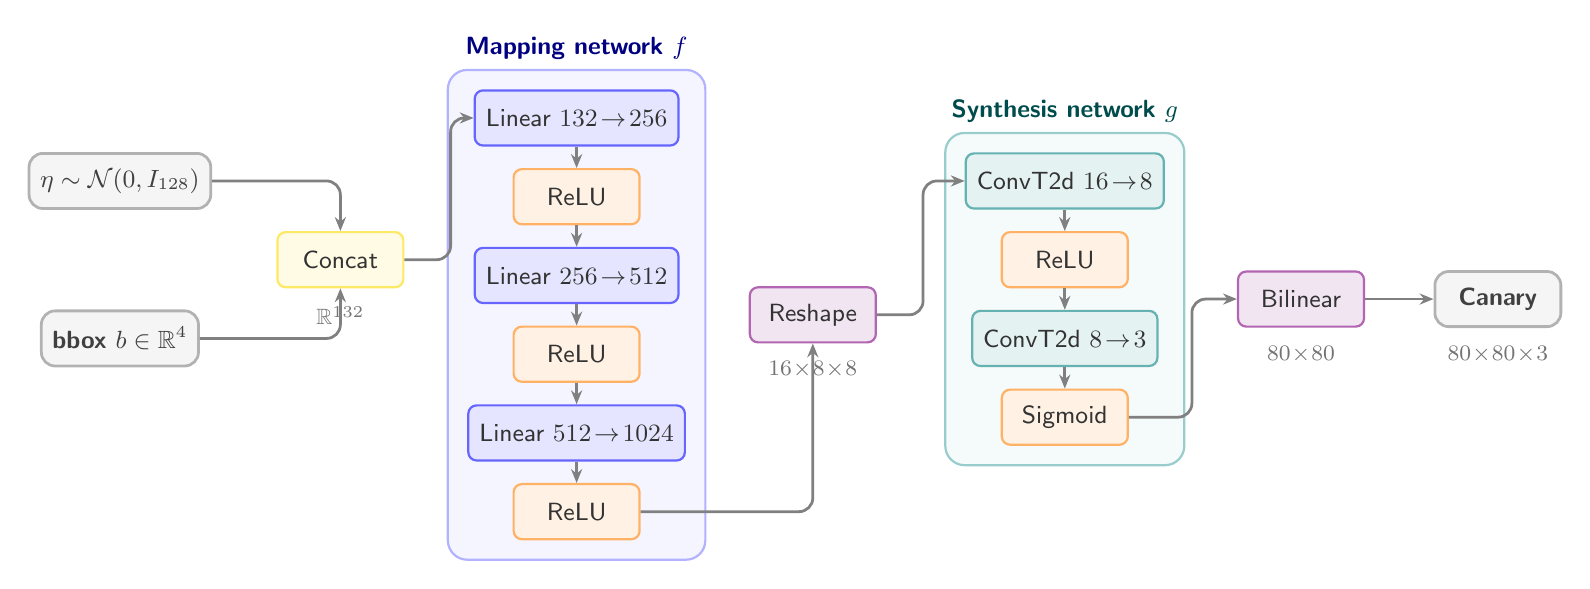
\begin{tikzpicture}[>=Stealth,
    % ---- styles ----
    B/.style={draw=#1!60, fill=#1!10, rounded corners=3pt,
              minimum width=1.6cm, minimum height=0.7cm,
              font=\small\sffamily, inner sep=4pt, line width=0.8pt,
              text=black!80},
    IO/.style={draw=black!30, fill=black!4, rounded corners=5pt,
               minimum width=1.6cm, minimum height=0.7cm,
               font=\small\sffamily\bfseries, inner sep=4pt, line width=1pt,
               text=black!75},
    D/.style={font=\footnotesize\sffamily\bfseries, text=black!55},
    A/.style={-{Stealth[length=5pt, width=4pt]}, color=black!50, line width=1pt,
              rounded corners=5pt},
    G/.style={rounded corners=7pt, inner sep=7pt, line width=0.8pt},
    T/.style={font=\small\sffamily\bfseries},
]

% ===== Column 1: Inputs =====
\node[IO] (noise) at (0, 1) {$\eta \sim \mathcal{N}(0, I_{128})$};
\node[IO] (bbox)  at (0,-1) {bbox $b \in \mathbb{R}^4$};
\node[B=yellow!80!orange] (cat) at (2.8, 0) {Concat};
\node[D, below=3pt of cat] {$\mathbb{R}^{132}$};

% Input to Concat
\draw[A] (noise.east) -| (cat.north);
\draw[A] (bbox.east)  -| (cat.south);

% ===== Column 2: Mapping network f =====
\node[B=blue]   (fc1) at (5.8, 1.8)  {Linear $132\!\to\!256$};
\node[B=orange] (r1)  at (5.8, 0.8)  {ReLU};
\node[B=blue]   (fc2) at (5.8,-0.2)  {Linear $256\!\to\!512$};
\node[B=orange] (r2)  at (5.8,-1.2)  {ReLU};
\node[B=blue]   (fc3) at (5.8,-2.2)  {Linear $512\!\to\!1024$};
\node[B=orange] (r3)  at (5.8,-3.2)  {ReLU};

\begin{scope}[on background layer]
    \node[G, draw=blue!30, fill=blue!4, fit=(fc1)(r1)(fc2)(r2)(fc3)(r3),
          label={[T, text=blue!50!black]above:Mapping network $f$}] (gm) {};
\end{scope}

% Concat -> mapping
\draw[A] (cat.east) -- (4.2,0) |- (fc1.west);
% Vertical within mapping
\foreach \a/\b in {fc1/r1, r1/fc2, fc2/r2, r2/fc3, fc3/r3}
    \draw[A] (\a) -- (\b);

% ===== Column 3: Reshape =====
\node[B=violet] (resh) at (8.8, -0.7) {Reshape};
\node[D, below=3pt of resh] {$16\!\times\!8\!\times\!8$};
% Mapping -> reshape: exit right, go across
\draw[A] (r3.east) -| (resh.south);

% ===== Column 4: Synthesis network g =====
\node[B=teal] (cv1) at (12.0, 1.0)  {ConvT2d $16\!\to\!8$};
\node[B=orange]     (r4)  at (12.0, 0.0)   {ReLU};
\node[B=teal] (cv2) at (12.0,-1.0)  {ConvT2d $8\!\to\!3$};
\node[B=orange]     (sig) at (12.0,-2.0)    {Sigmoid};

\begin{scope}[on background layer]
    \node[G, draw=teal!40, fill=teal!4, fit=(cv1)(r4)(cv2)(sig),
          label={[T, text=teal!60!black]above:Synthesis network $g$}] (gs) {};
\end{scope}

% Reshape -> synthesis: exit right, go up
\draw[A] (resh.east) -- (10.2,-0.7) |- (cv1.west);
% Vertical within synthesis
\foreach \a/\b in {cv1/r4, r4/cv2, cv2/sig}
    \draw[A] (\a) -- (\b);

% ===== Column 5: Output =====
\node[B=violet] (resize) at (15.0, -0.5) {Bilinear};
\node[D, below=3pt of resize] {$80\!\times\!80$};
\node[IO]       (out)    at (17.5, -0.5) {Canary};
\node[D, below=3pt of out] {$80\!\times\!80\!\times\!3$};

% Synthesis -> bilinear -> output
\draw[A] (sig.east) -- ++(0.8,0) |- (resize.west);
\draw[A] (resize) -- (out);

\end{tikzpicture}%
}% end resizebox
\end{center}

\vspace{0.1cm}
\small
\begin{columns}[t]
\column{0.32\textwidth}
\textbf{Input:} $z = [\eta \| b] \in \mathbb{R}^{132}$\\
128-d noise + 4-d bbox coords

\column{0.38\textwidth}
\textbf{Training:}\; $\min_\theta \lambda_c \mathcal{L}_{\text{canary}}(G_\theta) + \lambda_w \mathcal{L}_{\text{wood}}$\\
Gradients through frozen YOLOv8 $\to \theta$

\column{0.27\textwidth}
\textbf{Output:} $80\!\times\!80\!\times\!3$ patch\\
Inference: $\sim$5\,ms / canary
\end{columns}
\end{frame}

% ============================================================
\section{What Failed: Mode Collapse}
% ============================================================

\begin{frame}{Problem: Mode Collapse}
A single generator produces \textbf{identical outputs} regardless of input noise.

\vspace{0.1cm}
\begin{center}
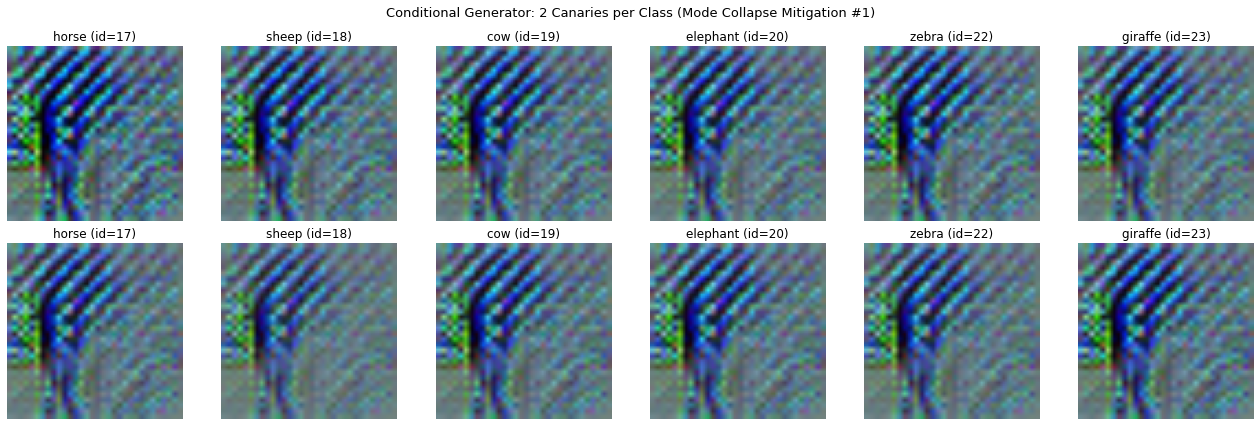
\includegraphics[width=0.7\textwidth]{fig1.png}
\end{center}

\vspace{0.1cm}
\textbf{Metrics:} Cosine similarity: \textbf{0.9957} (99.6\% identical), L2 distance: \textbf{5.40} (very low).

\vspace{0.1cm}
\textbf{Root cause:} Detection loss creates one strong attractor. Generator finds one pattern that YOLOv8 detects and produces it every time.
\end{frame}

\begin{frame}{Approach 1: Multi-Class Conditioning -- \textcolor{red}{FAILED}}
\begin{columns}
\column{0.55\textwidth}
\textbf{Idea:} Condition on 6 COCO classes (horse, sheep, cow, elephant, zebra, giraffe).

\vspace{0.2cm}
\textbf{What happened:}
\begin{itemize}
    \item Training \textbf{diverged}: benign loss UP (74 $\to$ 126), adversarial loss DOWN (87 $\to$ 70)
    \item 6-dim class one-hot too weak against 128-dim noise
    \item All classes produced identical canaries
\end{itemize}

\column{0.4\textwidth}
\begin{center}
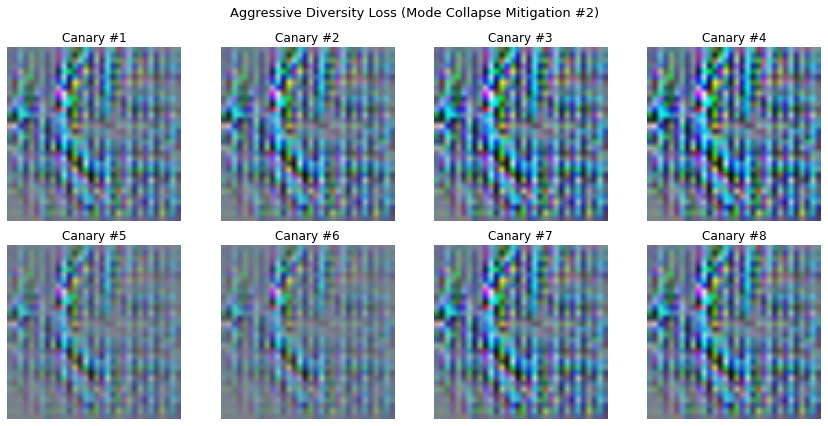
\includegraphics[width=\textwidth]{fig2.png}
\end{center}
\end{columns}
\end{frame}

\begin{frame}{Approach 2: Aggressive Diversity Loss -- \textcolor{red}{FAILED}}
\textbf{Idea:} Add cosine diversity penalty ($\lambda_{\text{div}} = 50$):
\begin{equation*}
    \mathcal{L}_{\text{total}} = \lambda_c \mathcal{L}_{\text{benign}} - \mathcal{L}_{\text{adv}} + \lambda_{\text{div}} \mathcal{L}_{\text{diversity}}
\end{equation*}

\vspace{0.3cm}
\textbf{Result:} No improvement.
\begin{itemize}
    \item Cosine similarity: still \textbf{0.9957}
    \item L2 distance: still \textbf{5.40}
    \item Detection loss attractor too strong for diversity penalty
    \item Increasing $\lambda_{\text{div}}$ further $\to$ training diverges (same as Approach 1)
\end{itemize}

\vspace{0.3cm}
\textbf{Key insight:} \textit{A single generator inherently wants to collapse.} You can't fight the loss landscape -- you must \textbf{sidestep} it.
\end{frame}

% ============================================================
\section{What Worked: Ensemble of Generators}
% ============================================================

\begin{frame}{Approach 3: Independent Ensemble -- \textcolor{green!60!black}{SUCCESS}}
\textbf{Idea:} Train $K$ independent generators with \textbf{different random seeds}. Each collapses to a \textbf{different mode}.

\vspace{0.1cm}
\begin{columns}
\column{0.55\textwidth}
\begin{center}
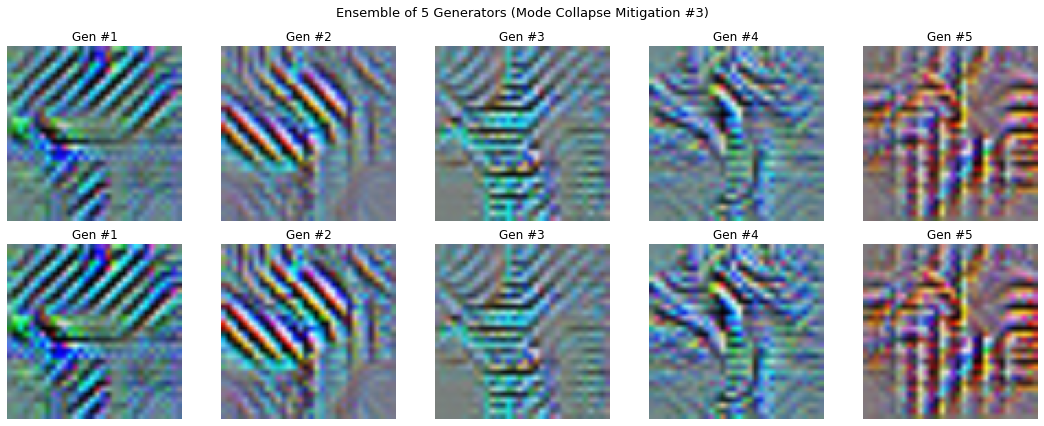
\includegraphics[width=\textwidth]{fig3.png}
\end{center}

\column{0.4\textwidth}
\textbf{Why it works:}
\begin{itemize}
    \item Different seed $\to$ different init
    \item Different init $\to$ different trajectory
    \item Different trajectory $\to$ different mode
    \item Diversity from \textbf{structure}, not loss
\end{itemize}

\vspace{0.2cm}
\textbf{5-gen proof of concept:}
\begin{itemize}
    \item L2: \textbf{29.56} (5.5$\times$ better)
    \item Training: $\sim$3.4 min/gen
\end{itemize}
\end{columns}
\end{frame}

% ============================================================
\section{Scaling to 1000 Generators on HPC}
% ============================================================

\begin{frame}{HPC Training: 4$\times$T4, 18 Hours, \$16}
\begin{columns}
\column{0.55\textwidth}
\textbf{Infrastructure:}
\begin{itemize}
    \item 4$\times$ NVIDIA T4 GPUs (16 GB each)
    \item Multi-GPU parallel script
    \item 250 generators per GPU
    \item Resume support (skip completed)
\end{itemize}

\vspace{0.3cm}
\textbf{How it works:}
\texttt{python train\_ensemble\_parallel.py \textbackslash}\\
\texttt{~~--n\_generators 1000 --n\_gpus 4}

\column{0.4\textwidth}
\begin{table}
\centering
\small
\begin{tabular}{lr}
\toprule
\textbf{Metric} & \textbf{Value} \\
\midrule
Generators & 1,000 \\
Epochs each & 50 \\
Time/gen & $\sim$3.4 min \\
Wall-clock & 18.04 hrs \\
GPUs & 4$\times$ T4 \\
Cost & $\sim$\$16 \\
Storage & 2.58 GB \\
\bottomrule
\end{tabular}
\end{table}
\end{columns}
\end{frame}

\begin{frame}{1000 Generators: Visual Snapshot}
\begin{center}
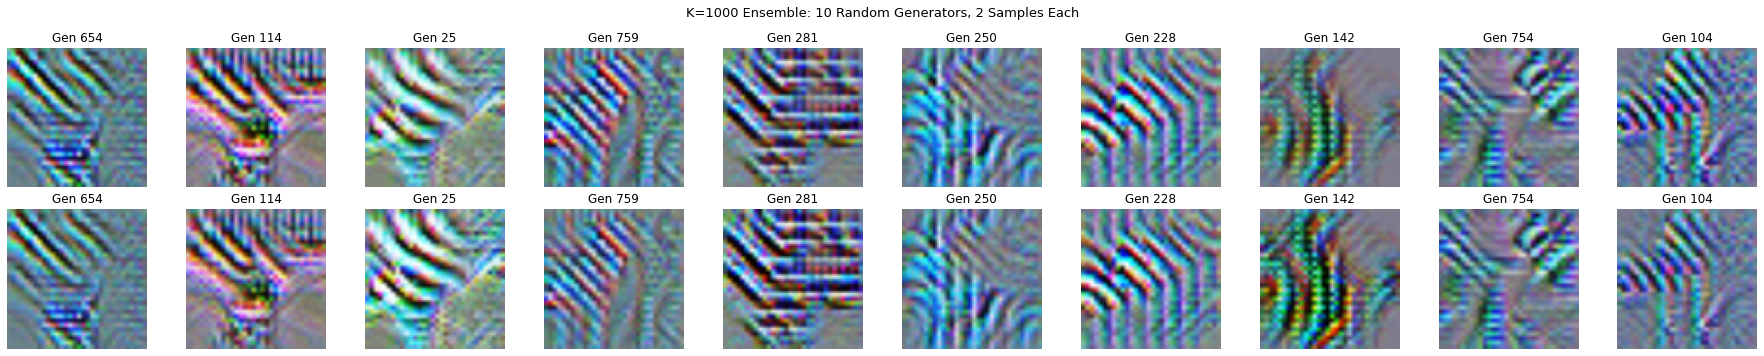
\includegraphics[width=0.85\textwidth]{fig4.png}
\end{center}

\vspace{0.3cm}
Each column = different generator from the pool of 1000.\\
Rows = two samples from the same generator (within-generator similarity).\\
Columns = different generators (between-generator diversity).
\end{frame}

% ============================================================
\section{Evaluation Results}
% ============================================================

\begin{frame}{Detection Performance: 1000-Gen Ensemble}
\begin{table}
\centering
\begin{tabular}{lcccccr}
\toprule
\textbf{Attack} & \textbf{Paper} & \textbf{Fixed} & \textbf{5-Gen} & \textbf{1000-Gen} & \textbf{FPR} & $\boldsymbol{\Delta}$ \\
\midrule
AdvPatch & 0.974 & 0.935 & 0.935 & 0.929 & 0.144 & $-$0.045 \\
UPC & 0.936 & 0.877 & 0.908 & 0.897 & 0.178 & $-$0.039 \\
TCEGA & 0.807 & 0.896 & 0.905 & \textbf{0.914} & 0.126 & \textcolor{green!60!black}{\textbf{+0.107}} \\
Natural & 0.871 & 0.900 & 0.929 & \textbf{0.923} & 0.127 & \textcolor{green!60!black}{\textbf{+0.052}} \\
\bottomrule
\end{tabular}
\end{table}

\vspace{0.3cm}
\begin{itemize}
    \item \textbf{Beats paper} on TCEGA (+10.7\%) and Natural (+5.2\%) -- the hardest attacks
    \item \textbf{Recall near-perfect:} AdvPatch 99.2\%, UPC 95.9\%, TCEGA 94.7\%, Natural 96.6\%
    \item \textbf{Tradeoff:} Higher FPR (0.126--0.178) vs.\ fixed canary (0.078--0.123)
    \item Fixed canary: F1=0.974 on AdvPatch \textbf{but breakable in 1.2 days on B200}
\end{itemize}
\end{frame}

% ============================================================
\section{Diversity Analysis}
% ============================================================

\begin{frame}{50 Canaries from 50 Different Generators}
\begin{center}
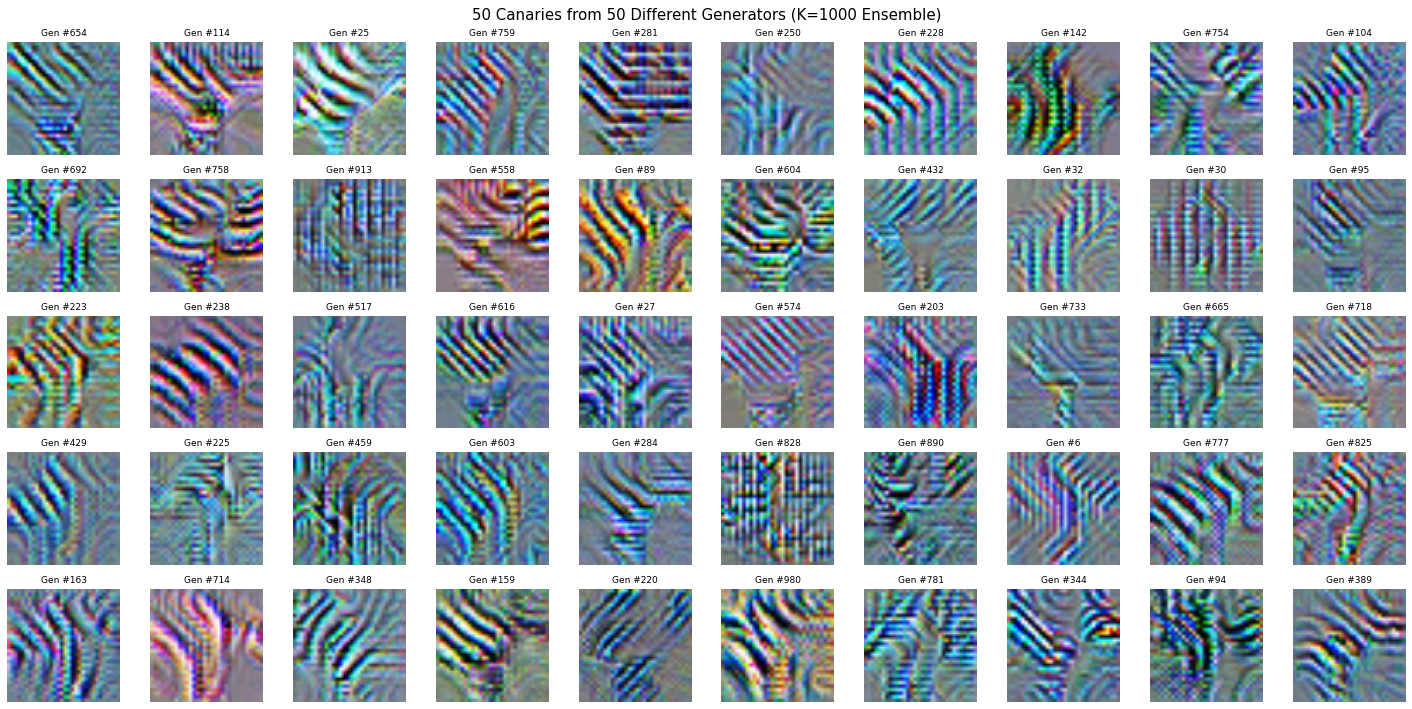
\includegraphics[width=0.78\textwidth]{fig5.png}
\end{center}

\vspace{0.1cm}
Every generator produces a \textbf{visually distinct} pattern: different orientations, colors, textures, densities.
\end{frame}

\begin{frame}{Diversity Metrics}
\begin{columns}
\column{0.55\textwidth}
\begin{table}
\centering
\small
\begin{tabular}{lrrr}
\toprule
\textbf{Config} & \textbf{L2} & \textbf{Cos Sim} & \textbf{Gain} \\
\midrule
Single gen & 5.40 & 0.9957 & 1$\times$ \\
5-gen & 29.56 & -- & 5.5$\times$ \\
\textbf{1000-gen} & \textbf{34.43} & \textbf{0.8821} & \textbf{6.4$\times$} \\
\bottomrule
\end{tabular}
\end{table}

\vspace{0.3cm}
\textbf{Detailed metrics (50 samples):}
\begin{itemize}
    \item Min L2: 21.37 (4$\times$ above collapsed baseline)
    \item Max L2: 46.19
    \item Mean (1 $-$ cosine): 0.1179
\end{itemize}

\column{0.4\textwidth}
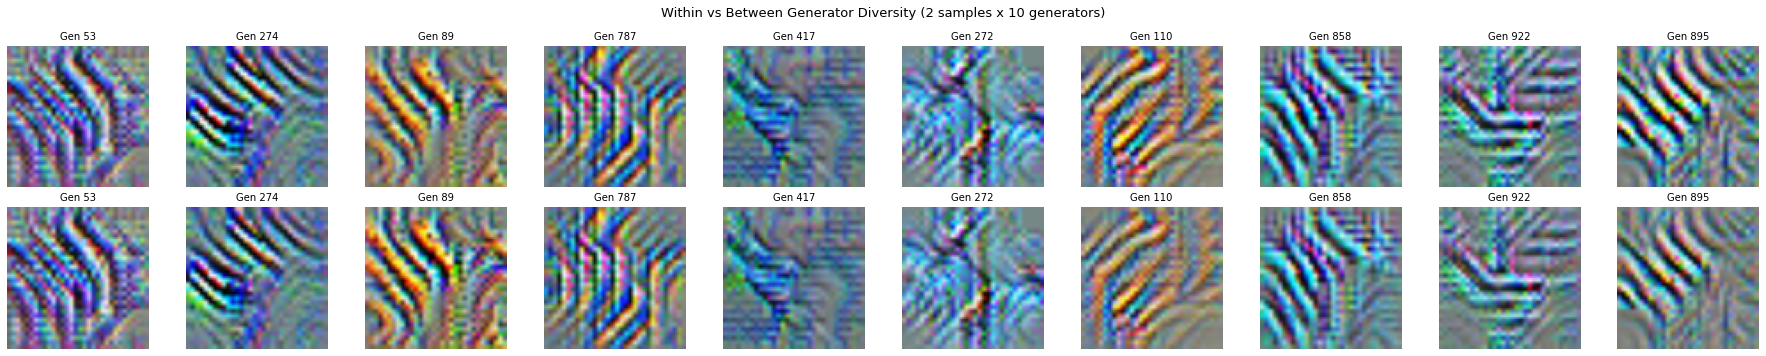
\includegraphics[width=\textwidth]{fig6.png}

\vspace{0.3cm}
\small Rows = same generator (similar).\\
Columns = different generators (diverse).\\
\textbf{Diversity comes from inter-generator variance, not from noise input.}
\end{columns}
\end{frame}

% ============================================================
\section{Theoretical Framework}
% ============================================================

\begin{frame}{Attacker's Optimization Problem}
Under the white-box threat model, the attacker knows everything. They must solve:

\begin{equation*}
    \delta^* = \arg\min_\delta \sum_{k=1}^{1000} \mathbb{E}_{z \sim \mathcal{N}(0, I_{128})} \left[ \mathcal{L}_{\text{AdvPatch}}(x + \delta) + \mathcal{L}_{\text{adv}}(c^k_z) \right]
\end{equation*}

\vspace{0.3cm}
\textbf{Plain English:} ``Find one t-shirt pattern that hides the person AND keeps ALL 1000 possible canaries visible, for EVERY possible random noise the defender might sample.''

\vspace{0.3cm}
\textbf{Three layers of difficulty:}
\begin{enumerate}
    \item \textbf{1000 generators:} Must satisfy 1000 different pattern families
    \item \textbf{Within-generator variation:} Each generator has internal $z$ variation
    \item \textbf{Fresh $z$ at inference:} Defender's actual $z$ has probability 0 of matching attacker's samples
\end{enumerate}
\end{frame}

\begin{frame}{Why More Compute Doesn't Help}
The attacker can only \textbf{approximate} the expectation by sampling $N$ noise vectors:
\begin{equation*}
    \hat{\delta} = \arg\min_\delta \frac{1}{N} \sum_{k=1}^{1000} \sum_{i=1}^{N} \left[ \mathcal{L}_{\text{AdvPatch}}(x + \delta) + \mathcal{L}_{\text{adv}}(c^k_{z_i}) \right]
\end{equation*}

\vspace{0.3cm}
\textbf{Why this fails:}
\begin{itemize}
    \item Approximation error: $O(1/\sqrt{N})$ -- to halve the error, need \textbf{4$\times$} the samples
    \item $N$ sampled points cover a \textbf{measure-zero} subset of $\mathbb{R}^{128}$
    \item Defender's actual $z^*$ matches attacker's samples with probability \textbf{exactly 0}
    \item Even with perfect average, patch only minimizes the \textbf{mean} -- individual unseen canaries can still detect
\end{itemize}

\vspace{0.3cm}
\textbf{More GPU $\neq$ solved.} Faster sampling doesn't change the fundamental coverage problem.
\end{frame}

% ============================================================
\section{Adversary Cost Analysis}
% ============================================================

\begin{frame}{Per-Term Attack Cost (from Original Paper)}
\textbf{Deriving the base unit:}
\begin{itemize}
    \item Original paper Table 9: 6 terms took 906 hours ($\sim$37 days) on RTX 3090
    \item Per-term cost: $906 / 6 \approx 151$ hours $\approx$ \textbf{6.2 days}
\end{itemize}

\vspace{0.3cm}
\textbf{How one iteration works:}
\begin{enumerate}
    \item Start with random patch pixels
    \item Forward pass through YOLOv8 with each canary combo
    \item Check: person hidden? canary visible?
    \item Backpropagate, nudge pixels
    \item Repeat thousands of times
    \item Each iteration: $K$ forward + $K$ backward passes
\end{enumerate}

\vspace{0.3cm}
\textbf{With $K=6$:} each iteration $\approx$ 600ms $\to$ converges in $\sim$37 days\\
\textbf{With $K=1000$:} each iteration $\approx$ 100s $\to$ converges in $\sim$\textbf{17 years} on RTX 3090
\end{frame}

\begin{frame}{Brute-Force Attack Cost}
\begin{table}
\centering
\begin{tabular}{lrrr}
\toprule
\textbf{Hardware} & \textbf{Speedup} & \textbf{Time (K=1000)} & \textbf{Feasible?} \\
\midrule
RTX 3090 & 1$\times$ & $\sim$17 years & \textcolor{red}{No} \\
B100 & $\sim$25$\times$ & $\sim$248 days & \textcolor{red}{No} \\
B200 & $\sim$32$\times$ & $\sim$194 days & \textcolor{red}{Impractical} \\
8$\times$ B200 & $\sim$253$\times$ & $\sim$24 days & \textcolor{orange}{State-level} \\
64$\times$ B200 & $\sim$2000$\times$ & $\sim$3 days & \textcolor{orange}{\$100K+} \\
\bottomrule
\end{tabular}
\end{table}

\vspace{0.3cm}
\textbf{Gambling attack (guess one generator):}
\begin{itemize}
    \item Probability: $1/1000 = 0.1\%$
    \item Expected attempts: 500
    \item Expected time on B200: \textbf{600 days}
    \item \textbf{Only works for ONE image} -- next image picks a different generator
\end{itemize}
\end{frame}

\begin{frame}{Defender vs.\ Attacker: The Cost Asymmetry}
\begin{table}
\centering
\large
\begin{tabular}{lll}
\toprule
& \textbf{Defender} & \textbf{Attacker} \\
\midrule
\textbf{Cost} & \textcolor{green!60!black}{\$16} & \textcolor{red}{\$34,000+} \\
\textbf{Time} & \textcolor{green!60!black}{18 hours} & \textcolor{red}{194 days} \\
\textbf{Result} & All images protected & Breaks all (until retrain) \\
\textbf{Repeatable?} & Yes, \$16 each & No, starts from zero \\
\bottomrule
\end{tabular}
\end{table}

\vspace{0.5cm}
\begin{center}
\Large
\textbf{Cost ratio:} $\dfrac{C_{\text{attacker}}}{C_{\text{defender}}} = \dfrac{6.2 \text{ days}}{3.4 \text{ min}} \approx$ \textcolor{accent}{\textbf{2,629$\times$}}

\vspace{0.3cm}
\normalsize
This ratio is \textbf{hardware-independent}.\\Both sides benefit equally from faster GPUs.
\end{center}
\end{frame}

% ============================================================
\section{The Killer Move: Retrainability}
% ============================================================

\begin{frame}{The Killer Move: Retrain and Invalidate}
\textbf{Scenario:} Attacker spends 6 months and \$34,000 on a B200. Finally breaks all 1000 generators.

\vspace{0.5cm}
\textbf{Defender runs:}
\texttt{python train\_ensemble\_parallel.py --n\_generators 1000}
With new random seeds.

\vspace{0.5cm}
\textbf{18 hours and \$16 later:} All 1000 generators are different.\\
Attacker's 6 months of work is \textbf{completely invalidated}.\\
They must \textbf{restart from zero}.

\vspace{0.5cm}
\begin{center}
\large
The defender can \textbf{rotate the defense at will} for negligible cost.\\
The attacker \textbf{always loses} the economic war.
\end{center}
\end{frame}

% ============================================================
\section{Limitations}
% ============================================================

\begin{frame}{Limitations}
\begin{enumerate}
    \item \textbf{Higher FPR:} Ensemble FPR (0.126--0.178) $>$ fixed canary (0.078--0.123). More diversity = some canaries less reliable on clean images.

    \vspace{0.2cm}
    \item \textbf{Mode collapse within generators:} Each generator still collapses internally. Diversity comes from the ensemble, not from $z$ variation.

    \vspace{0.2cm}
    \item \textbf{Diversity plateau:} L2 only improved 1.16$\times$ from 5$\to$1000 generators (29.56$\to$34.43). Architecture may be saturating.

    \vspace{0.2cm}
    \item \textbf{No empirical adaptive attack:} Cost projections are theoretical (scaled from original paper). We did not run actual adaptive attacks against 1000 generators.

    \vspace{0.2cm}
    \item \textbf{Single detector, single dataset:} YOLOv8 on VOC07 only. Extension to other detectors is straightforward but not tested.
\end{enumerate}
\end{frame}

% ============================================================
\section{Summary}
% ============================================================

\begin{frame}{Summary}
\textbf{Gap identified:} FFF security is hardware-dependent, not complexity-dependent.

\vspace{0.3cm}
\textbf{What we tried and failed:}
\begin{itemize}
    \item Multi-class conditioning $\to$ training diverged
    \item Aggressive diversity loss $\to$ no effect (cosine = 0.9957)
\end{itemize}

\vspace{0.3cm}
\textbf{What worked:} Ensemble of 1000 independent generators.

\vspace{0.3cm}
\textbf{Key results:}
\begin{itemize}
    \item F1: 0.897--0.929. Beats paper on TCEGA (+10.7\%) and Natural (+5.2\%)
    \item Diversity: L2=34.43, cosine=0.8821 (6.4$\times$ improvement)
    \item Defender: \$16, 18 hours. Attacker: \$34K+, 194 days on B200
    \item Cost ratio: \textbf{2,629$\times$} (hardware-independent)
    \item Retrainable overnight for \$16 -- invalidates all attacker work
\end{itemize}
\end{frame}

\begin{frame}{The Bottom Line}
\begin{center}
\Large
\vspace{1cm}
Fixed canary: F1 = 0.974 on AdvPatch\\
\textcolor{red}{Breakable in 1.2 days on a B200.}

\vspace{1cm}
1000-gen ensemble: F1 = 0.929 on AdvPatch\\
\textcolor{green!60!black}{\textbf{Requires $\sim$194 days on a B200 to break.}}

\vspace{1cm}
Defender invalidates everything overnight for \textbf{\$16}.
\end{center}
\end{frame}

\begin{frame}
\begin{center}
\Huge
\textbf{Thank You}

\vspace{1cm}
\Large
Questions?
\end{center}
\end{frame}

\end{document}
